\chapter{Medidor de Presión}
Utilizando un sensor de presión $MDX2010DP$ se diseñó e implementó en PCB un circuito un medidor de presión utilizando un amplificador de instrumentación que cumpla con las especificaciones de la Tabla \ref{e4:tab_specs}, alimentado por una única fuente de tensión.

\begin{table}[ht]
\begin{center}
\begin{tabular}{||c|c||c|c|c||}
\hline
Característica				&Símbolo	&Min	&Máx	&Unidades \\
\hline
Tensión de salida mínima	&$V_{min}$	&0		&0		&$V$ \\
Tensión de salida máxima	&$V_{max}$	&3.1	&3.3	&$V$ \\
Tensión de alimentación		&$V_{DC}$	&10		&15		&$V$ \\
\hline
\end{tabular}
\caption{Especificaciones para el diseño del Medidor de Presión}
\label{e4:tab_specs}
\end{center}
\end{table}

\section{Diseño}
\subsection{Sensor de Presión}
A partir de la hoja de datos del MPX2010DP, se tomó en cuenta la información en la Tabla \ref{e4:tab_sensor_specs} para el diseño del medidor de presión.

\begin{table}[ht]
\begin{center}
\begin{tabular}{||c|c||c|c|c|c||}
\hline
Característica				&Símbolo				&Min		&Typ	&Máx		&Unidades \\
\hline
Rango de Presión			&$P_{OP}$				&0		&-	&10		&$V$ \\
Tensión de alimentación		&$V_{DC}$				&0		&10	&16		&$V$ \\
Tope de Escala				&$V_{FSS}$			&24		&25	&26		&$mV$ \\
Sensibilidad				&$\Delta V / \Delta P$ 	&-		&2.5	&-		&$mV/kPa$\\
\hline
\end{tabular}
\caption{Especificaciones del Sensor de Presión}
\label{e4:tab_sensor_specs}
\end{center}
\end{table}

\subsection{Amplificador de Instrumentación}
Para el Amplificador de Instrumentación (A.I.) se utilizó el diseño de dos amplificadores operacionales ilustrado en la Figura \ref{e4:fig_amp_inst}.
Es posible calcular la ganancia del circuito completo observando que el primer bloque del A.I. se trata de un circuito amplificador no inversor, por lo que su ganancia estará dada por la expresión (\ref{e4:eq_A1}) donde $a_1$ es la ganancia a lazo abierto del amplificador operacional U1 y $v_o'$ es su tensión de salida.

\begin{figure}[ht]
\begin{center}
\begin{circuitikz}[american voltages]
\draw
(0,0) node[op amp] (opamp1) {U1}
(6,-0.5) node[op amp] (opamp2) {U2}
(opamp1.-) to[R=$R_1$,*-] ++(-3,0) to ++(0,-2) node[ground]{GND}
(opamp1.+) to[sinusoidal voltage source=$V_1$] ++(0,-3) node[ground]{GND}
(opamp1.-) to ++(0,1) to[R=$R_2$] ++(3,0) to[short,-*] ++(0,-1.5)
(opamp1.out)to[R=$R_3$,-*] (opamp2.-)
(opamp2.+) to[sinusoidal voltage source=$V_2$] ++(0,-2.5) node[ground]{GND}
(opamp2.-) to ++(0,1) to[R=$R_4$] ++(3,0) to[short] ++(0,-1.5) node[right]{$v_{out}$} to (opamp2.out)
;
\end{circuitikz}
\caption{Amplificador de Instrumentación}
\label{e4:fig_amp_inst}
\end{center}
\end{figure}

\begin{equation}
%\mathlarger{
A_1 = \frac{v_o'}{V_1} = \left(1+ \frac{R_2}{R_1}\right) \cdot \frac{1}{1 + \frac{1+R_2/R_1}{a_1}}
%}
\label{e4:eq_A1}
\end{equation}

Por otro lado, en la segunda sección del A.I. la salida del amplificador operacional U2 puede calcularse aplicando el principio de superposición entre la tensión $v_o'$ y $V_2$:

\begin{equation}
%\mathlarger{
v_{out} = V_2 \cdot \left(1 + \frac{R_4}{R_3}\right) \cdot \frac{1}{1 + \frac{1+R_4/R_3}{a_2}} + v_o' \cdot \left(- \frac{R_4}{R_3}\right) \cdot \frac{1}{1 + \frac{1+R_4/R_3}{a_2}}
%}
\label{e4:eq_v_out}
\end{equation}

Operando con las expresiones (\ref{e4:eq_A1}) y (\ref{e4:eq_v_out}) se obtiene para la tensión de salida del A.I.

\begin{equation}
%\mathlarger{
v_{out} = \left(1 + \frac{R_4}{R_3}\right) \cdot \frac{1}{1 + \frac{1+R_4/R_3}{a_2}} \cdot \left[ V_2 - V_1 \cdot \frac{1+ R_2/R_1}{1+R_3/R_4} \cdot \frac{1}{1 + \frac{1+R_4/R_3}{a_1}} \right]
%}
\label{e4:eq_v_out_a_fin}
\end{equation}

Finalmente, considerando que los amplificadores operacionales tienen una ganancia infinita ($a_1 \cap a_2 \rightarrow \infty$) se obtiene la expresión simplificada 

\begin{equation}
%\mathlarger{
v_{out} = \left(1 + \frac{R_4}{R_3}\right) \cdot \left[ V_2 - V_1 \cdot \frac{1+ R_2/R_1}{1+R_3/R_4} \right]
%}
\label{e4:eq_v_out_a_inf}
\end{equation}

A partir de la expresión (\ref{e4:eq_v_out_a_inf}) se oberva que el A.I. se encuentra balanceado cuando se cumple la condición

\begin{equation}
%\mathlarger{
1+\frac{R_2}{R_1} = 1+\frac{R_3}{R_4} \Rightarrow \frac{R_2}{R_1} = \frac{R_3}{R_4}
%}
\label{e4:eq_cond_bal}
\end{equation}

Tomando la expresión \eqref{e4:eq_v_out_a_inf} se pueden calcular las ganancias a modo común ($A_{CM}$) y a modo diferencial ($A_{DM}$)

\begin{equation}
%\mathlarger{
A_{CM} = 1 - \frac{R_4}{R_3} \cdot \frac{R_2}{R_1}
%}
\label{e4:eq_A_cm}
\end{equation}

\begin{equation}
%\mathlarger{
A_{DM} = \frac{R_4}{R_3} + \frac{1}{2} \cdot \left(1+ \frac{R_4}{R_3} \cdot \frac{R_2}{R_1}\right)
%}
\label{e4:eq_A_dm}
\end{equation}

Cuando se cumple la condición de balance descripta en \eqref{e4:eq_cond_bal} se obtiene que idealmente $A_{CM_B} = 0$ y $A_{DM_B} = 1+R_4/R_3$.

\begin{equation}
%\mathlarger{
CMRR=10\log\left(\frac{A_{DM}}{A_{CM}}\right)
%}
\end{equation}

\subsection{Selección de Componentes}
Tomando en cuenta los datos de las Tablas \ref{e4:tab_specs} y \ref{e4:tab_sensor_specs}, se busca que $A_{DM_B}$ esté típicamente dada por la expresión \eqref{e4:eq_r4_r3}. Además, se buscó que se cumpla la condición de balance del A.I. y por lo tanto se tomaron $R_1=R_4$ y $R_3 = R_2$.

\begin{equation}
%\mathlarger{
1+ \frac{R_4}{R_3}=\frac{\SI{3.2}{\volt}}{\SI{25}{\milli\volt}}= 128 \Rightarrow R_4=127 R_3
%}
\label{e4:eq_r4_r3}
\end{equation}
 
\begin{table}[ht]
\begin{center}
\begin{tabular}{||c|c|c|c||}
\hline
Resistencia	&	Valor &	Tolerancia & Real\\
\hline	
$R_1$	&	$150\si{\kilo\ohm} + 2.2\si{\kilo\ohm}$	&	$1\%$	&	$149\si{\kilo\ohm} + 2.20\si{\kilo\ohm}$ \\
$R_2$	&	$1.2\si{\kilo\ohm}$	&	$1\%$	&	$1.198\si{\kilo\ohm}$ \\
$R_3$	&	$1.2\si{\kilo\ohm}$	&	$1\%$	&	$1.199\si{\kilo\ohm}$ \\
$R_4$	&	$150\si{\kilo\ohm} + 2.2\si{\kilo\ohm}$	&	$1\%$	&	$149\si{\kilo\ohm} + 2.20\si{\kilo\ohm}$ \\
\hline
\end{tabular}
\end{center}
\caption{Valores de las resistencias}
\label{e4:tab_res_vals}
\end{table}

Dado que se busca evitar que el Amplificador de Instrumentación esté desbalanceado, se utilizaron resistencias con $1\%$ de tolerancia.

Además, como amplificador operacional se utilizó el \textit{LM833} dado que contiene dos amplificadores operacionales dentro del mismo circuito integrado. Esto permite asumir que ambos \textit{opamps} tienen los mismos parámetros de operación. En este caso, una impedancia de entrada alta (no especificada en la hoja de datos), y bajos niveles de ruido. Este último es importante dado que no se desea insertar ruido durante las etapas de amplificación a la señal que tiene 

\newpage
\section{Simulación}

Con los componentes seleccionados en la Tabla \ref{e4:tab_res_vals} se construyó el circuito en \textit{LTspice XVII} de modo que se puedan simular por separado las ganancias en modo común y en modo diferencial como se ilustra en las Figuras
%\ref{e4:fig_spice_cm_ac},
\ref{e4:fig_spice_cm_dc},
%\ref{e4:fig_spice_dm_ac}
 y 
\ref{e4:fig_spice_dm_dc}
.
\begin{figure}[!ht]
\begin{center}
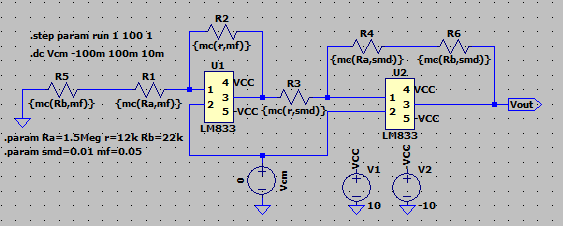
\includegraphics[width=\linewidth]{res/spice/spice_cm_dc_sch.png}
\caption{Esquemático de la simulación en Modo Común en CC}
\label{e4:fig_spice_cm_dc}
\end{center}
\end{figure}

\begin{figure}[!ht]
\begin{center}
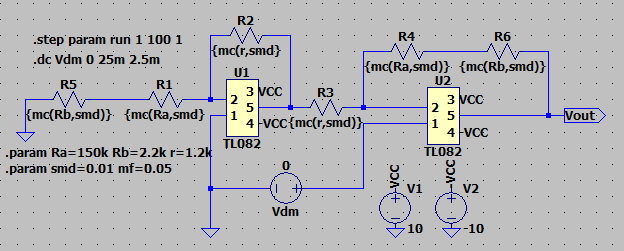
\includegraphics[width=\linewidth]{res/spice/spice_dm_dc_sch.png}
\caption{Esquemático de la simulación en Modo Diferencial en CC}
\label{e4:fig_spice_dm_dc}
\end{center}
\end{figure}

Se observa en los resultados del análisis de Montecarlo en las Figuras \ref{e4:fig_spice_cm_dc_mc} y \ref{e4:fig_spice_dm_dc_mc} que la tensión de salida del Modo Común no excede en módulo los $30 \si{\milli\volt}$ y la tensión de salida del Modo Diferencial se encuentra dentro del rango de tensiones de salida buscadas.

%\begin{figure}[!ht]
%\begin{center}
%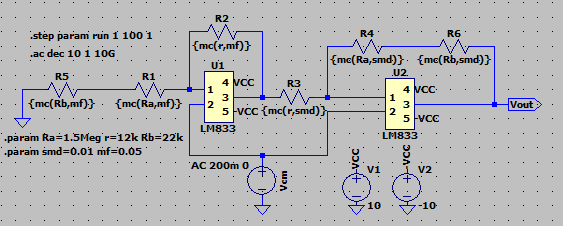
\includegraphics[width=\linewidth]{res/spice/spice_cm_ac_sch.png}
%\caption{Esquemático de la simulación en Modo Común en CA}
%\label{e4:fig_spice_cm_ac}
%\end{center}
%\end{figure}

%\begin{figure}[!ht]
%\begin{center}
%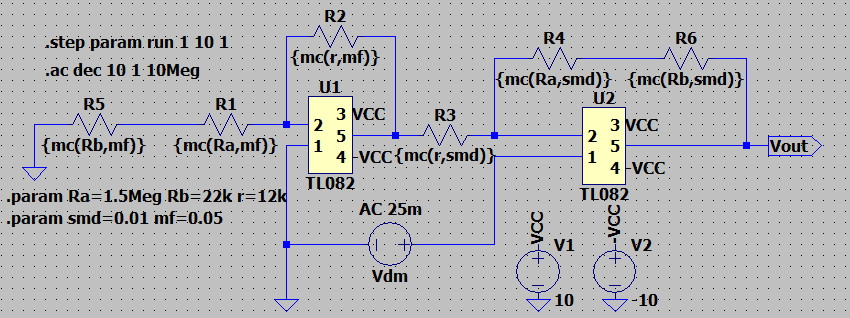
\includegraphics[width=\linewidth]{res/spice/spice_dm_ac_sch.png}
%\caption{Esquemático de la simulación en Modo Diferencial en CA}
%\label{e4:fig_spice_dm_ac}
%\end{center}
%\end{figure}

\section{Resultados}

A partir de las simulaciones en \textit{LTSpice} se obtuvieron los gráficos de las Figuras 

\begin{figure}[!ht]
\begin{center}
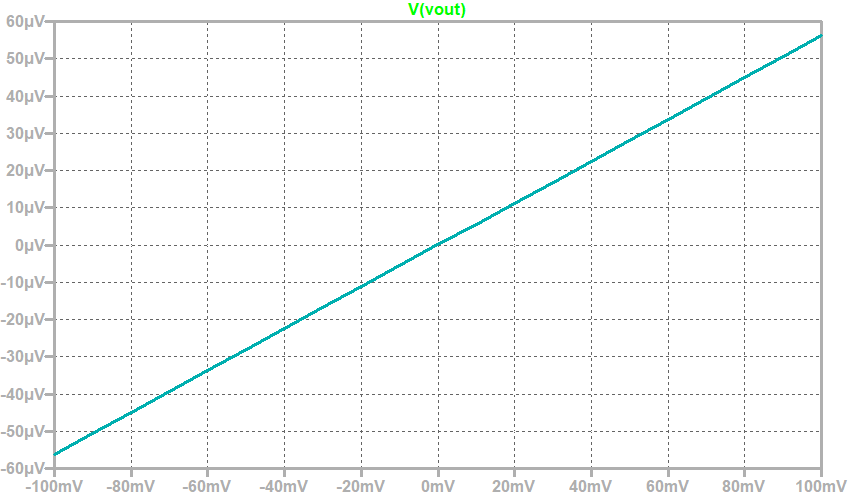
\includegraphics[width=0.9\linewidth]{res/spice/spice_cm_dc.png}
\caption{Resultado de la simulación en Modo Común en CC}
\label{e4:fig_spice_cm_dc_res}
\end{center}
\end{figure}

\begin{figure}[!ht]
\begin{center}
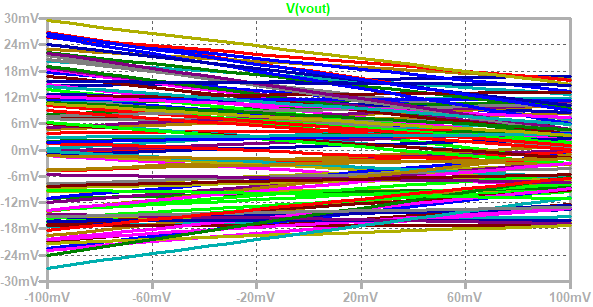
\includegraphics[width=0.85\linewidth]{res/spice/spice_cm_dc_mc.png}
\caption{Resultado del Análisis de Montecarlo en Modo Común en CC}
\label{e4:fig_spice_cm_dc_mc}
\end{center}
\end{figure}

\begin{figure}[!ht]
\begin{center}
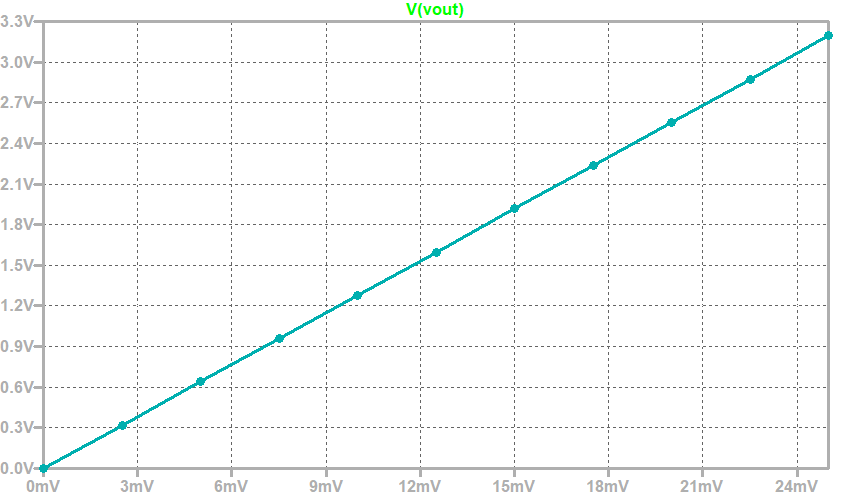
\includegraphics[width=0.85\linewidth]{res/spice/spice_dm_dc.png}
\caption{Resultado de la simulación en Modo Diferencial en CC}
\label{e4:fig_spice_dm_dc_res}
\end{center}
\end{figure}

\begin{figure}[!ht]
\begin{center}
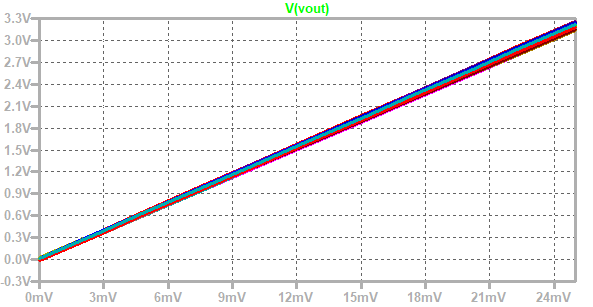
\includegraphics[width=0.85\linewidth]{res/spice/spice_dm_dc_mc.png}
\caption{Resultado del Análisis de Montecarlo en Modo Diferencial en CC}
\label{e4:fig_spice_dm_dc_mc}
\end{center}
\end{figure}

\pagebreak
\pagebreak
\pagebreak

\section{Construcción del PCB}

Siguiendo el esquemático de la Figura \ref{e4:fig_pcb_sch} se contruyó el PCB con la estructura vista en la Figura \ref{e4:fig_pcb_route}.

\begin{figure}[!ht]
\begin{center}
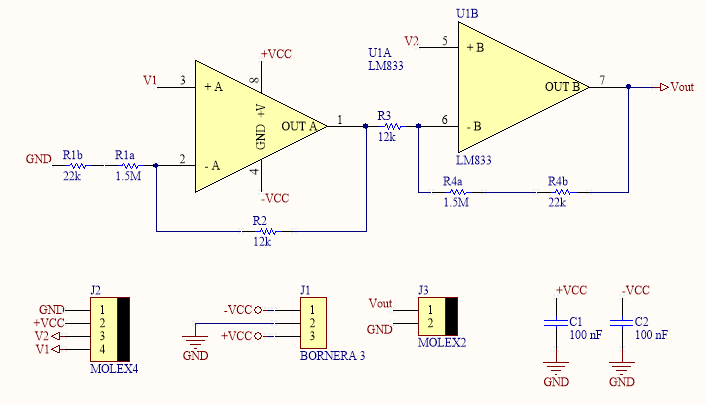
\includegraphics[width=0.7\linewidth]{res/altium/sch.png}
\caption{Esquemático del Amplificador de Instrumentación}
\label{e4:fig_pcb_sch}
\end{center}
\end{figure}

\begin{figure}[!ht]
\begin{center}
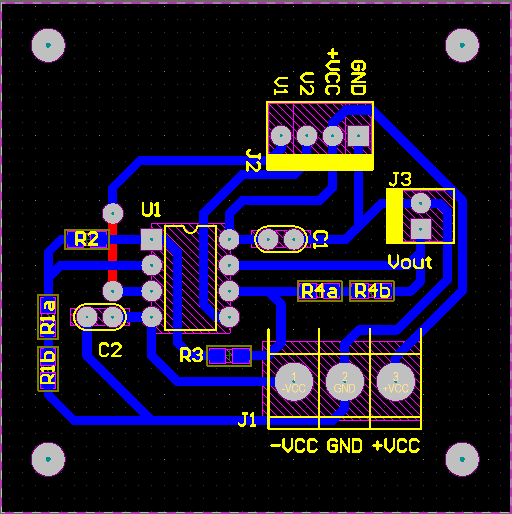
\includegraphics[height=7cm]{res/altium/pcb.png}
\caption{Routeado del PCB del Amplificador de Instrumentación}
\label{e4:fig_pcb_route}
\end{center}
\end{figure}

\newpage

Utilizando los valores de componentes de especificados en el Cuadro \ref{e4:tab_res_vals}, se calcula que las ganancias serán las dadas en el Cuadro \ref{e4:tab_A}.

\begin{table}[!ht]
\begin{center}
\begin{tabular}{||c|c||}
\hline
Parámetro	&Valor	\\
\hline
$A_{CM}$	&$8.3403\times	10^{-4}$	\\
$A_{DM}$	&$127.1047$	\\
$CMRR$	&$51.82 dB$	\\
\hline
\end{tabular}
\caption{Parámetros del Amplificador de Instrumentación}
\label{e4:tab_A}
\end{center}
\end{table}

\section{Método de Medición}
Se utilizó un generador de onda $V_{in}$ para excitar el circuito con diferentes niveles de tensión continua. 
Para medir la ganancia en modo común, se conectaron las terminales de entrada V1 y V2 a la terminal positiva del generador de señales y la terminal negativa a tierra.
Como se espera que en el modo común la señal se atenúe, se utilizaron valores de tension tales que la salida esté sobre el piso de ruido de $100 \si{\milli\volt}$.

Para medir la ganancia en modo diferencial, se conectó la terminal V1 a tierra y la terminal V2 a la terminal positiva del generador de señales.
Como se espera que en el modo diferencial la señal sea amplificada, se utilizaron valores de tension tales que la salida no sature.

A partir de estos valores se calculó el la razón de rechazo al modo común.

\section{Análisis de Resultados}

Se midió la ganancia en modo diferencial y se registró en la Tabla \ref{e4:tab_vdm}.
Cuando la tensión a modo diferencial era $V_{DM}=0$, la tensión de salida medida fue de $V_{off}=0.073\si{\volt}$. La ganancia a modo común no pudo ser medida, dado que cualquier valor

\begin{table}[ht]
\begin{center}
\begin{tabular}{||c|c|c|c|c||}
\hline
$V_{in DM}$(mV)&$V_{out DM}$(V)&$A_{DM}$(V/V)&$V_{out}-V_{off}$&$A_{DM2}$\\
\hline
60	&7.724	&128.73	&7.651	&127.517	\\
50	&6.45	&129		&6.377	&127.54	\\
40	&5.17	&129.25	&5.097	&127.425	\\
30	&3.893	&129.77	&3.82	&127.33	\\
25	&3.244	&129.76	&3.171	&126.84	\\
20	&2.619	&130.95	&2.546	&127.3	\\
15	&1.972	&131.47	&1.899	&126.6	\\
10	&1.35	&135		&1.277	&127.7	\\
5	&0.695	&139		&0.622	&124.4	\\
\hline
\end{tabular}
\caption{Mediciones a modo Diferencial}
\label{e4:tab_vdm}
\end{center}
\end{table}

En promedio, la ganancia a Modo Diferencial cuando se elimina el \textit{offset} fue de $A_{DM_{AVG}}=126.96$ veces.

Dado que la tensión de salida a Modo Común fue demasiado baja como para ser medida, ya que la tensión máxima que pueden entregar los generadores de onda es de $10V$, para el cálculo del rechazo al modo común se tomó como valor de la ganancia a Modo Común su valor teórico $A_{CM}=8.34\times 10^{-4}$.

A partir de estos dos datos, se calculó el valor del Rechazo al Modo Común, $CMRR = 51.98 dB$.


Es necesario mencionar la exisencia de un nivel de tensión presente constantemente a lo largo de la medición. Esto evita que pueda cumplirse estríctamente la condición de que el Analizador de Instrumentación devuelva $0 V$ cuando no existe una diferencia de tensión entre ambas terminales de entrada.

En primer lugar, esto puede resolverse utilizando amplificadores operacionales con menores niveles de ruido introducidor por el integrado mismo.

En segundo lugar, otra manera de resolver la existencia de esta tensión de \textit{offset} es cambiando el Amplificador de Instrumentación por uno donde la configuración de las entradas sea simétrica y existe un Amplificador Operacional adicional el cual permite regular los niveles de Tensión de \textit{offset}.

En tercer lugar, en lugar de utilizar resistencias en serie para conseguir la razón necesaria para obtener la ganancia a Modo Diferencial deseada, se puede incluir un resistor variable para modificar la ganancia del Amplificador de Instrumentación. Esto permite que la ganancia pueda ser recalibrada cada vez que sea necesario y disminuye la cantidad de componentes, los cuales introducen ruido térmico.

\section{Limitación de Tensión}

Para proteger cualquier dispositivo que se encuentre a la salida del Amplificador de Instrumentación, se aplicó el circuito mostrado en la Figura \ref{e4:fig_v_lim}.

\begin{figure}[ht]
\begin{center}
\begin{circuitikz}[american voltages]
\draw
(0,0) node[ground]{GND} to[zzDo,l=$3.3V$,-*] ++(0,3) node[right]{$V_{Z}'$}
to[R=$R_Z$,-*] ++(-4,0) node[left]{$v_{o}$}
;
\end{circuitikz}
\caption{Circuito Limitador de Tensión}
\label{e4:fig_v_lim}
\end{center}
\end{figure}

Dado que el Diodo Zener tiene una potencia máxima de $0.5 \si{\watt}$ y se busca que la tensión máxima sea de $3.3 \si{\volt}$
\begin{equation*}
I_{Z}=0.5 \si{\watt}/3.3 \si{\volt}\approx 0.150 \si{\ampere}
\end{equation*}

Sin embargo, la corriente máxima de salida del amplificador operacional es de $20 mA$, por lo tanto, para no quemar la resistencia:

\begin{equation*}
R<\frac{P_R}{{I_o}^2}\approx 0.125 W/{(0.02\si{\ampere})}^2=312.5 \si{\ohm}
\end{equation*}

Se escogió una resistencia de $10\si{ohm}$ de tal forma que no provocara una caída de tensión tal que la tensión de salida del circuito quede por debajo de los $3.1V$. En principio, se probó este sistema con un diodo Zener de $3.3 V$; sin embargo, se notó que con esta configuración la tensión del diodo fue de $3.45 V$ cuando era activado. Considerando esto, se utilizó un diodo de $3.0V$ para mantener los niveles de tensión al menos debajo de los $3.3V$.

\section{Presión en una columna de agua}
%Medicion de la presion dentro de un tubo de agua y se obtuvieron los resultados.
\subsection{Método de Medición}
Se colocó un extremo de un tubo a la entrada de presión positiva del sensor de presión, y el otro extremo se insertó hasta la base de la probeta. Luego se añadió una cantidad de agua y se midieron la altura de la columna de agua dentro de la probeta, la altura del agua dentro del tubo y la tensión de salida del amplificador de instrumentación. Esto se repitió para distintas cantidades de agua.

\begin{figure}[ht]
\begin{center}
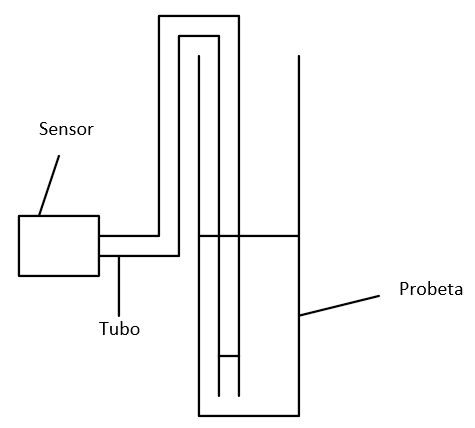
\includegraphics[scale=0.5]{./res/probeta.png}
\caption{Sistema de medición de la presión}
\end{center}
\end{figure}

\subsection{Resultados}
\begin{table}[ht]
\begin{center}
\begin{tabular}{||c|c|c|c|c|c||}
\hline
h en el Caño (cm) &h en el Tubo (cm)&$\Delta h (m)$&$V_{out} (V)$& V sin offset & P (kPa)\\
\hline
0&0&0,000&0,237&0,000&0,000\\
15&5&0,100&0,543&0,306&1,000\\
33&18&0,150&0,627&0,390&1,500\\
59&25&0,340&1,216&0,979&3,400\\
82&31&0,510&1,752&1,515&5,100\\
93&34&0,590&1,961&1,724&5,900\\
112&38&0,740&2,453&2,216&7,400\\
119&40&0,790&2,623&2,386&7,900\\
130&42&0,880&2,905&2,668&8,800\\
133&43&0,900&2,955&2,718&9,000\\
141&45&0,960&3,170&2,933&9,600\\
148&46&1,020&3,334&3,097&10,200\\
\hline
\end{tabular}
\caption{Resultados de la medición con la probeta de agua.}
\end{center}
\end{table}

\subsection{Análisis de Resultados}

\begin{align*}
P &= F/A \\
F &= m \times g = \rho \cdot V \times g = \rho \cdot h \cdot A \cdot g\\
P &= \rho \cdot g \cdot h [Pa] = \frac{\rho g}{1000}\cdot h [kPa]
\end{align*}

\begin{equation}
\Delta P [kPa]= \frac{\rho g}{1000}\cdot \Delta h
\label{e4:eq_p}
\end{equation}

De \eqref{e4:eq_p} se puede observar cómo la presión ejercida por una columna de líquido solo depende de su altura y densidad. En el caso del agua, como se conoce $\rho = 1000 kg \cdot m^{-3}$ y $g \approx 10 m\cdot s^{-2}$, para una diferencia de altura de $1 m$ se espera medir una presión de $10 \si{\kilo\pascal}$.

\begin{figure}
\begin{center}
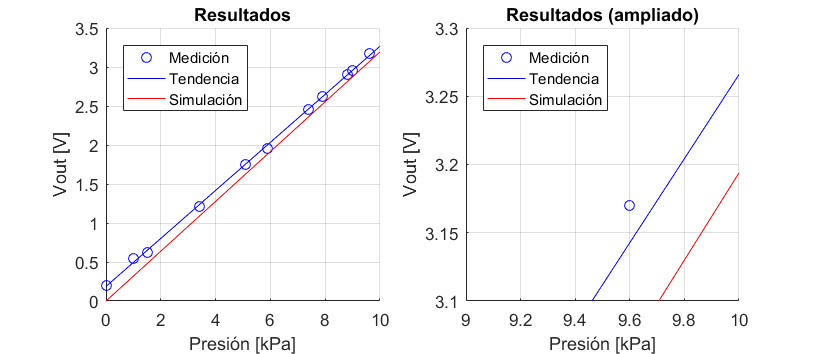
\includegraphics[scale=0.6]{./res/medysim.png}
\caption{Resultados de la Medición de la presión en la probeta con agua}
\label{e4:fig_p}
\end{center}
\end{figure}

El corrimiento entre la tensión de salida del amplificador de instrumentación observada en la Figura \ref{e4:fig_p} se debe a la tensión de \textit{offset} mencionada previamente.

Teniendo en cuenta el resultado de \eqref{e4:eq_p} puede calcularse el volume de agua en cualquier recipiente cilíndrico o prismático, cuya base se conozca el área, sin necesidad de alterar físicamente el amplificador de instrumentación. Este cálculo no necesita cambios en el sistema electrónico del circuito. Por otro lado, si el líquido fuese cambiado, el valor de la densidad será distinto, y por lo tanto la salida del Amplificador de Instrumentación deberá ser utilizada con un cálculo distinto para calcular el volume de líquido en recipiente. Una vez más, esto no requerirá cambios en el sistema electrónico del circuito.

Aunque no son necesarios cambios en el circuito electrónico del Amplificador de Instrumentación, sí es necesario cambiar cómo se utiliza el sensor de presion. En lugar de utilizar este método experimental, es necesario conectar el sensor directamente a la base del recipiente, permitiendo una medición directa de la presión ejercida por el líquido sobre la base de su recipiente. Sólo debe conectarse la entrada de presión positiva porque esta es la única que cuenta con una membrana protectora para que no ingresen líquidos al sistema interno del sensor.

\section{Conclusión}

Utilizar el tipo de Amplificador de Instrumentación de la Figura \ref{e4:fig_amp_inst} trae ventajas y desventajas. Por un lado, tiene la ventaja de que se utilizan sólo dos amplificadores operacionales y típicamente requiere menos componentes para construir el amplificador de instrumentación. Además, al contener sólamente \textit{opamps}, existen menos etapas donde se puede introducir ruido al sistema.

Por otro lado, existirán complicaciones con los niveles de ruido introducidos por los integrados y los componentes. Al ser esta configuración no simétrica, es posible que estas señales de ruido introducidas por la presencia de los componentes electrónicos alteren la tensión de salida.

Finalmente, se recomienda utilizar diseños que permitan la recalibración del amplificador de instrumentación, de manera que este pueda ser utilizado con diferentes tipos de sensores que no compartan los niveles de tensión con el MPX2010DP utilizado.